\documentclass{article}
\usepackage{textcomp}
\usepackage{url}
\usepackage{geometry}
\usepackage[cmex10]{amsmath}
\usepackage{amssymb}
\usepackage{topcapt}
\usepackage{booktabs}
\usepackage{times}
\usepackage{bm}
\usepackage{algorithmic}
\usepackage{algorithm}
\usepackage{array}
\usepackage{color}
%\usepackage[nomarkers]{endfloat/endfloat}
\usepackage[outerbars]{changebar}

\usepackage[sort&compress]{natbib}
\bibpunct{[}{]}{,}{n}{,}{,}


\usepackage{authblk}
\usepackage[font=small]{caption}

\renewcommand{\baselinestretch}{1.5}
\textheight=8.5in
\textwidth=6.5in
\oddsidemargin=0in
\headsep=0.0in
\headheight=0.0in
%\parskip=12pt

\let\citepleft=(
\let\citepright=)

\usepackage{bm}
\usepackage{url}
\usepackage{todonotes}
% collection of notation 
\newcommand{\bmag}{$\vert B_1^+\vert$} % JBM b1-selective character
\newcommand{\bfullt}{b_{total}(t)}
\newcommand{\bext}{b_{ex}(t)}
\newcommand{\bbst}{b_{bs}(t)}


\newif\ifmarkedup
\markeduptrue

\ifmarkedup
	\newcommand{\revbox}[1]{\marginpar{\framebox{#1}}}
\else
	\newcommand{\revbox}[1]{}
	\renewcommand{\textcolor}[1]{}
\fi

 
%%%%%%%%%%%%%%%%%%%%%


%%%%%%%%%%%%%%%%%%%%%
\begin{document}
%%TC:ignore
\title{\vspace{-2cm}Selective Excitation Localized by the Bloch-Siegert Shift}
\date{}

\author[1,2]{Jonathan B. Martin}
\author[1,2]{Sai Abitha Srinivas}
\author[1,2]{Christopher E. Vaughn}
\author[2]{Heng Sun}
\author[3,4]{Mark A. Griswold}
\author[1,2,5]{William A. Grissom}


\affil[1]{\small Vanderbilt University Institute of Imaging Science, Nashville, Tennessee, USA}
\affil[2]{\small Department of Biomedical Engineering, Vanderbilt University, Nashville, Tennessee, USA}
\affil[3]{\small Department of Radiology, Case Western Reserve University, Cleveland, Ohio, USA}
\affil[4]{\small Department of Biomedical Engineering, Case Western Reserve University, Cleveland, Ohio, USA}
\affil[5]{\small Department of Electrical Engineering, Vanderbilt University, Nashville, Tennessee, USA}
\maketitle

\vfill
\noindent

\noindent
\textit{Address correspondence to:} \\
  Jonathan B. Martin \\
  1161 21st Ave. South, MCN AA-1105, Nashville, TN 37232-2310 \\
  jonathan.b.martin@vanderbilt.edu\\


\noindent
This work was supported by NIH grants R01 EB 030414 and R01 EB 016695

\noindent
Submitted to \textbf{\textit{Magnetic Resonance in Medicine}} as a Research Article.

\noindent
Approximate word count: 207 (Abstract) $\sim$4900 (Body)\\

\noindent
\textbf{Key Words:} RF pulse design, Selective RF excitation, Bloch-Siegert shift, RF encoded MRI, Multiphoton, low-field MRI

\clearpage

\begin{abstract}

\noindent\textbf{Purpose:} To perform $B_1^+$-selective excitation using the Bloch-Siegert shift for spatial localization. \\
\textbf{Methods:} 
A $B_1^+$-selective excitation is produced by an RF pulse consisting of two summed component pulses: an off-resonant pulse that induces a $B_1^+$-dependent Bloch-Siegert frequency shift and a frequency-selective excitation pulse.
The passband of the pulse can be tailored by adjusting the frequency content of the frequency-selective pulse, 
as in conventional $B_0$ gradient-localized excitation. Fine magnetization profile control is achieved by using the Shinnar-Le Roux algorithm to design the frequency-selective excitation pulse.
Simulations analyze the pulses' robustness to off-resonance, 
their suitability for multi-echo spin echo pulse sequences, 
and how their performance compares to that of rotating-frame selective excitation pulses. 
The pulses are evaluated experimentally on a 47.5 mT MRI scanner using an RF gradient transmit coil.
Multiphoton resonances produced by the pulses are characterized and their distribution across $B_1^+$ predicted.\\
\textbf{Results}
With correction for varying $B_1^+$ across the desired profile, 
the new pulses produce selective excitation with the specified profile characteristics. The pulses are shown to be robust against off-resonance and suitable for multi-echo pulse sequences.
Experimental profiles closely match simulated patterns. \\
\textbf{Conclusion}
The Bloch-Siegert shift can be used to perform $B_0$-gradient-free selective excitation,
enabling the excitation of slices or slabs in RF gradient-encoded MRI.\\
\\
\textbf{Key Words:} RF pulse design, Selective RF excitation, Bloch-Siegert shift, RF encoded MRI, Multiphoton, low-field MRI
\end{abstract}

\noindent

\clearpage



%%%%%%%%%%%%%%%%%%%%%%%%%%%%%%%%------- INTRODUCTION -------%%%%%%%%%%%%%%%%%%%%%%%%%%%%%%%%
\section*{Introduction}
Spatially selective excitation is a necessity in nearly all magnetic resonance imaging. 
Objects under investigation are usually large and 3-dimensional, 
whereas the region from which signal is desired is typically restricted to a slice, slab, or limited volume. 
Spatial selectivity is conventionally achieved by pairing a frequency-selective radiofrequency (RF) 
pulse with gradients of the main magnetic field $B_0$. 
In the one-dimensional case, 
a linear field gradient $G_z$ superimposed on the main magnetic field produces a spatially-dependent shift in spins' resonant frequencies $f(x) = -(\gamma/2\pi)(B_0 + zG_z)$ \cite{Mansfield1977Multi-planarEchoes}. 
Simultaneously applying an RF pulse from a transmit coil with a homogeneous 
transmit field selectively excites spins that are frequency shifted by the gradient to within the bandwidth $\Delta\omega$ of the RF pulse (Fig. 1a). Within this framework, 
well-developed methods can be applied to design RF pulses that meet 
target magnetization profile characteristics \cite{Conolly1986OptimalProblem, Pauly1991ParameterAlgorithm}. 
While the use of $B_0$ gradients for localizing excitation is effective and widely adopted, 
there are also serious challenges that accompany $B_0$ gradients. 
Gradient hardware is expensive and occupies a large portion of a scanner's bore area, 
constraining scanner design; gradient switching is loud and induces peripheral nerve stimulation, 
compromising patient comfort; and eddy currents and concomitant non-linear magnetic fields induced by gradients require correction to prevent image artifacts \cite{Bernstein1998ConcomitantCorrection, Spees2011QuantificationGradients}.

\par Imaging with magnitude or phase gradients of the RF transmit field ($B_1^+$) rather than the static $B_0$ main field has long been investigated as an alternative \cite{Hoult1979RotatingZeugmatography,Sharp2010MRIGradients,Kartausch2014SpatialEffect, Torres2021B1-gradientbasedEchoes} to $B_0$ gradient encoding. 
$B_1^+$ gradients can be switched in near-negligible time without acoustic noise, eddy currents, 
or peripheral nerve stimulation resulting from large $dB/dt$ \cite{Canet1997RadiofrequencyExperiments}. 
Though radiofrequency heating effects can limit the use of RF-encoded imaging at high main field strengths, 
tissue heating is low enough at lower field strengths to allow for long pulse trains or even continuous application of RF energy \cite{Kartausch2014SpatialEffect}. 

\par However, replacing $B_0$ gradients with RF magnitude gradients in an imaging system introduces a new challenge: 
how to spatially localize excitation utilizing only the RF transmit field itself. 
A number of methods exist which exploit an inhomogeneous transmit field for spatial discrimination, 
such as early techniques for localized spectroscopy in $B_1^+$ gradients utilizing composite $180^\circ$ hard pulses \cite{Tycko1984SpatialInversion, Shaka1984SpatiallyPulses}. 
These pulse trains achieve a rudimentary degree of spatial localization but require multiple FID acquisitions to define the ROI and do not provide strict profile definition. 
Another approach, the related depth pulse sequence technique, 
requires a smaller number of FID acquisitions and is somewhat more robust against off-resonance than composite pulses, 
but similarly provides little control over the excitation profile \cite{Bendall1983DepthCoils}. 
A third method proposed by Hoult is rotating-frame $B_1^+$-selective excitation (RFSE) 
by means of an RF pulse with constant $B_{1,x}$ and modulated $B_{1,y}$ \cite{Hoult1980NMRPulses}. 
These pulses selectively excite magnetization based on the strength of the $B_{1,x}$ component. 
The selectivity of the rotating frame method was improved with DANTE-inspired implementations using trains of alternating $B{1,x}$ and $B_{1,y}$ pulses \cite{Karczmar1988ShapedSimulations,Maffei1991SliceCoil}, 
early soft-pulse designs \cite{Hedges1988TheResults}, 
and a later recasting of the problem as a rotated Shinnar-Le Roux (SLR) design which enabled 
pulse designers to meet target slice profile characteristics in $B_1^+$ \cite{Grissom2014B1+-selectiveAlgorithm}. 
Although this most recent method finally provided fine control of the excitation profile, 
these pulses suffer from a number of challenges, 
including unintended excitation at low $B_1^+$ with off-resonance and potential RF amplifier distortions due to the pulses' high power demands and strict envelope area requirements \cite{Grissom2014B1+-selectiveAlgorithm}. 

\par This work describes a class of $B_1^+$-selective RF pulses that use the Bloch-Siegert shift \cite{Bloch1940MagneticFields} to localize excitation. 
The Bloch-Siegert shift is a temporary shift in the resonance frequency of a nucleus, produced by the application of an off-resonant RF field. 
The size of the frequency shift induced by the off-resonant RF field depends on the frequency offset of the applied pulse and the strength of the RF field. 
This property has allowed the Bloch-Siegert shift to be used for mapping $B_1^+$ fields in MRI \cite{Sacolick2010B1Shift} and calibrating decoupling field strength in NMR \cite{Hosur1983AShifts,Hung2020UsingSample}. More recently, the phenomenon has been exploited as an encoding mechanism for $B_0$ gradient-free imaging \cite{Kartausch2014SpatialEffect, Zhipeng2014FrequencyShift, Wan2017PhaseTransmit}. However, the authors are not aware of the Bloch-Siegert shift previously being used for excitation localization. Preliminary aspects of the pulse design algorithm were presented by the authors in Ref. \cite{Martin2021Bloch-SiegertPulses}.

\par The proposed $B_1^+$-selective pulses comprise the summation of 1) a far-off-resonant Bloch-Siegert frequency-shift-inducing pulse, 
and 2) a frequency-selective excitation pulse. 
The two pulses work in analog to the paired $B_0$ z gradient and frequency-selective excitation pulse used in conventional imaging slice selection. 
The Bloch-Siegert pulse creates a nonlinear frequency gradient that varies with $B_1^+$ field strength, 
and the frequency-selective pulse is designed to have a bandwidth that excites a range of $B_1^+$'s of interest (Fig. 1b). 
If the transmit coil generates a spatially inhomogeneous $B_1^+$ field,
the $B_1^+$ selectivity of the summed pulse translates to spatial selectivity. 

\par The primary resonance used for excitation by the proposed pulses is the Bloch Siegert-shifted single-photon resonance, initially at the Larmor frequency before being shifted. 
However, the new pulse class is reliant on the simultaneous application of two off-resonant pulses in the xy plane, 
which also produces additional multiphoton resonances \cite{Zur1983MultiphotonI=1/2, Krauss1986Four-fieldI=1/2}. 
These multiphoton resonances are distributed across $B_1^+$, 
resulting in additional bands of weaker excitation at other transmit field strengths.
Although imaging techniques that use multiphoton resonances for excitation have recently been demonstrated \cite{Han2020MultiphotonImplementation}, 
these additional resonances are here regarded as nuisances and their prediction and mitigation is discussed.

\par In the following, the design of the two component pulses that make up a Bloch-Siegert-localized $B_1^+$-selective excitation pulse is described. 
Although there are many choices for both the off-resonant Bloch-Siegert-shift inducing pulse and the frequency-selective pulse, 
this work focuses on the promising combination of an amplitude- and frequency-swept off-resonant pulse 
and an SLR frequency-selective pulse which allows the designer to directly specify and 
analytically trade off pulse and $B_1^+$ profile parameters \cite{Pauly1991ParameterAlgorithm}. 
The design algorithm for these two pulses is analytic, simple, and fast. 
Simulations show the pulses' suitability for selective excitation, inversion, and refocusing. 
Off-resonance behavior is simulated and shown to be predictable and similar to that of conventional spatially slice-selective excitation pulses, 
without the out-of-band excitation produced by the RFSE pulses of Ref \cite{Grissom2014B1+-selectiveAlgorithm}. 
Selective excitation is experimentally demonstrated on a low-field 47.5 mT MRI scanner 
with a gradient solenoid transmit-receive coil.

%%%%%%%%%%%%%%%%%%%%%%%%%%%%%%%%------- Pulse Design -------%%%%%%%%%%%%%%%%%%%%%%%%%%%%%%%%
\section*{Pulse Design}
The design of a Bloch-Siegert $B_1^+$-selective excitation (BSSE) pulse comprises the design of two distinct component pulses: 
1) an off-resonant pulse, $\bbst$, which produces a $B_1^+$-dependent shift in resonant frequencies via the Bloch-Siegert effect, 
and 2) a frequency-selective SLR pulse, $\bext$, which excites a desired $B_1^+$ passband.
Although these two pulses could be transmitted by separate coils, 
we here assume that they are generated together by the same transmit coil, 
so they are complex-summed once individually designed, i.e.,
\begin{equation*}
\bfullt = \bbst + \bext
\end{equation*}

\subsection*{Component Pulse 1: The Bloch-Siegert Shift-Inducing Pulse} 
In the absence of externally applied RF,
the magnetic resonance frequency is the Larmor frequency, $\omega_0 = \gamma B_0$. 
If an RF field is applied with amplitude $B_1^+$ and frequency offset 
$\omega_{off}$ relative to $\omega_0$, 
then a Bloch-Siegert frequency shift of the resonance is produced, given by \cite{Ramsey1955}:
\begin{equation}
\omega_{bs}(B_1^+, \omega_{off}) \approx -\omega_{off}\left(\sqrt{1+\left(\frac{\gamma B_1^+}{\omega_{off}}\right)^2}-1\right).
\label{eq:bsshift}
\end{equation}
This shift is away from the frequency of the applied off-resonance RF, i.e.,
a positive $\omega_{off}$ results in a negative $\omega_{bs}$.

\par The Bloch-Siegert shift-inducing pulse is defined as an amplitude- and phase-modulated function
\begin{equation}
    \bbst = A_{bs}(t)e^{i \phi_{bs}(t)},
\end{equation}
where $\phi_{bs}(t) = \int_{-T/2}^{t} \Delta\omega_{rf}(t') dt'$ 
is the time integral of the pulse's time-varying frequency modulation $\Delta \omega_{rf}(t)$,
and $T$ is the pulse duration. 
For $A_{bs}(t)$ we use a Fermi pulse
which was previously used in Ref. \cite{Sacolick2010B1Shift}   
to produce a large BS frequency shift with little out-of-band excitation. 
The Fermi envelope provides an additional benefit for this application: 
its plateau results in a constant
$\omega_{bs}$ for the majority of the pulse duration, 
which simplifies the design of the $\bext$ pulse in $\S 2.2$ 
so long as $\bext$ is restricted to be nonzero only on the plateau.
Thus for $A_{bs}(t)$ a normalized Fermi pulse is used which is  
centered at $t=0$:
\begin{equation}
    A_{bs}(t) =     	\frac{1}{1+e^{\frac{|t|-t_0}{a}}}
    \label{eq:abs}
\end{equation}
where $t_0$ and $a$ are parameters with units of seconds 
that control the duration of the pulse and the width of the transition, respectively. The duration of this Fermi pulse is $T = 2 t_0 + 13.81 a$.
To ensure that $\bext$ is only nonzero during the plateau when $A_{bs}(t) \approx 1$, 
we derive from Eq. \ref{eq:abs} that $t_0$ should be set to:
\begin{equation}
    t_0 = \frac{T_{ex}}{2}-a\ln{\left(\frac{1}{A_{th}}-1\right)},
\end{equation} 
where $T_{ex}$ is the duration of $\bext$ required to excite the desired bandwidth
and $A_{th}$ is a user-specified constant. 
This $t_0$ setting 
creates a central plateau in the Fermi envelope of duration $T_{ex}$ with $A_{bs}(t) \geq A_{th}$. 
Herein, all pulse designs used $a = 6\times10^{-5}$ s and $A_{th}$ = 0.95.

\par A modification is made 
to the conventional constant frequency-offset Fermi by starting and ending the pulse's FM waveform
far-off resonance and sweeping adiabatically towards and away from the central constant frequency offset $\omega_{off}$. 
This modification spin-locks the magnetization during the Fermi's amplitude sweeps, reducing undesired excitation by $A_{bs}(t)$ \cite{Garwood2001TheNMR, KhalighiAdiabaticMapping}.
The analytic adiabatic sweep of Ref. \cite{KhalighiAdiabaticMapping} is used, 
with modification to allow for time-varying $A_{bs}(t)$ rather than the constant AM waveform assumed in the previous work. The first half of the symmetric frequency sweep is given by:
\begin{equation}
    \begin{array}{ll}
    \Delta\omega_{sweep}(t) = \frac{\gamma A_{bs}(t)}{\sqrt{\left(1-\frac{\gamma A_{bs}(t)}{K}t\right)^{-2}-1}}, & t \in \left(0, T/2\right), \end{array}
\end{equation}
where $T$ is the duration of the full $A_{bs}(t)$ waveform and $K$ is a design parameter which allows a tradeoff between the maximum offset of the frequency sweeps and undesired excitation by $A_{bs}(t)$.
$K = 0.2$ was used for all pulses in this work, 
which produces a maximum frequency offset of $\sim$10-30 kHz given $\omega_{off}\sim5-20$ kHz, the practical range for most pulses. 
The full FM waveform with constant frequency plateau $\omega_{off}$ is then given by:
\begin{equation}
	\Delta\omega_{rf}(t) = \left\{ \begin{array}{rl} 	-\Delta\omega_{sweep}(t+T/2)+\max(\Delta\omega_{sweep}(t))+\omega_{off}, & -T/2<t<0, \\ 
	-\Delta\omega_{sweep}(T/2 - t)+\max(\Delta\omega_{sweep}(t))+\omega_{off}, & 0 \leq t<T/2, \end{array} \right.
\end{equation}
An example of an amplitude- and frequency-modulated $\bbst$ is shown in Fig. 2.
Note that the frequency modulation of this pulse is positive for all $t$, 
producing a negative Bloch-Siegert frequency shift for all $B_1^+$. 
As a result, the frequency-selective excitation pulse described in the next section is 
modulated to a negative frequency relative to Larmor, 
to excite the desired $B_1^+$ passband.

\subsection*{Component Pulse 2: The Frequency-Selective SLR Excitation Pulse}
For a given desired passband between field strengths $B_{1,L}^+$ and $B_{1,H}^+$, 
the bandwidth of resonant frequencies that must be excited by the frequency selective SLR pulse $b_{ex}(t)$ is:
\begin{equation}
B = \omega_{bs}(B_{1,L}^+, \omega_{off})-\omega_{bs}(B_{1,H}^+, \omega_{off}).
\label{eq:bandwidth}
\end{equation}
$\bext$ must further be frequency modulated to the center of the passband,
which has frequency:
\begin{equation}
\omega_{cent} = \frac{1}{2} \left(\omega_{bs}(B_{1,L}^+, \omega_{off}) + \omega_{bs}(B_{1,H}^+, \omega_{off})\right).
\label{eq:centerfreq}
\end{equation}
The Shinnar Le-Roux (SLR) pulse design algorithm is used to design $\bext$ since
it allows for direct design of pulses to meet design constraints including bandwidth ($B$), 
duration ($T_{ex}$), flip angle ($\theta$), transition width, 
and magnetization profile ripple ($\delta_1^e$ and $\delta_2^e$) \cite{Pauly1991ParameterAlgorithm}. 
Based on these parameters, 
SLR designs a pair of polynomials that are 
transformed to the discretized excitation pulse by the inverse SLR transform. 
Given the designer's choice of time-bandwidth product $T_{ex}B$, 
the duration of the excitation pulse $T_{ex}$ is determined by $B$.
The RF pulse output by SLR is interpolated to the target dwell time
and scaled to produce the desired flip angle $\theta$ for the $B_1^+$ 
at its passband center, based on the relationship:
\begin{equation}
    \theta = \gamma \Delta_t B_1^+(\omega_{cent}) \sum_{i=0}^{N-1} A_{ex}(t_i),
    \label{eq:fa_scaling}
\end{equation}
where $\Delta_t$ is the dwell time, 
$N$ is the number of time points in the pulse,
and $A_{ex}(t)$ is the baseband RF pulse waveform generated by SLR after interpolating
it to the target dwell time.
$B_1^+(\omega_{cent})$ is derived from Eq. \ref{eq:bsshift} after rearranging it 
to give the $B_1^+$ producing a Bloch-Siegert shift of $\omega$ during an RF pulse with frequency offset $\omega_{off}>0$: 
\begin{equation}
    B_1^+(\omega) \approx \frac{\omega_{off}}{\gamma}\sqrt{\left(1-\frac{\omega}{\omega_{off}}\right)^2-1}.
\label{eq:b1bsshift}
\end{equation}
After scaling $A_{ex}(t)$ to the desired flip angle, 
$b_{ex}(t)$ is obtained by frequency modulating it to $\omega_{cent}$.
The final pulse is then:
\begin{equation}
    b_{ex}(t) = A_{ex}(t) e^{i \omega_{cent} t}.
\end{equation}
Before summing $b_{ex}(t)$ with $b_{bs}(t)$, $b_{ex}(t)$ is zero-padded to match the full duration $T$ of $\bbst$.
An example $\bext$ for $T_{ex}B=4$ and $\theta=90^\circ$ is shown in Figure 2. 

\par However, under the assumption that both $\bext$ and $\bfullt$ are played from the same transmit coil, 
 $\bext$ will produce a sloped magnetization profile (or a distorted profile, in the case of 180$^\circ$ excitation) due to the fact that $\bext$ is played out slightly weaker than designed at passband locations where $B_1^+ <  B_1^+(\omega_{cent})$ and slightly stronger than designed where $B_1^+ > B_1^+(\omega_{cent})$. 
The degree of distortion will depend on the width of the passband relative to its center, $(B_{1,H}^+ - B_{1,L}^+) / B_1^+(\omega_{cent})$, and is therefore more pronounced for wide passbands and center positions closer to zero. Modifications can be made to the SLR algorithm to correct for these distortions, and the procedure adopted is outlined in Fig. 3a.
For small-tip and $90^\circ$ excitation, 
the distortion is approximately compensated by scaling the SLR algorithm's $B_N(\omega)$ 
polynomial by the inverse of the transmit field strength corresponding to each frequency $\omega$ in the profile,
with normalization to $B_1^+(\omega_{cent})$, prior to applying the inverse SLR transform:
\begin{equation}
    B_N(\omega) \leftarrow \frac{B_1^+(\omega_{cent})}{B_1^+(\omega + \omega_{cent})}B_N(\omega).
\end{equation}
For $180^\circ$ inversion or refocusing,
profile distortion cannot be corrected with this analytic method. 
Instead, as described in $\S 3.2$ an iterative optimization of the RF pulse is used to alleviate 
profile distortion caused by varying $B_1^+$.

\subsection*{Overall Pulse Design Procedure} 
The overall pulse design procedure is to first select the $B_1^+$ passband edges $B_{1,H}^+$ and $B_{1,L}^+$,
the excitation pulse's SLR algorithm parameters and flip angle, 
and the BS pulse's frequency offset $\omega_{off}$.
With these parameters, the SLR pulse is designed, interpolated to the target dwell time,
scaled to the desired flip angle, and frequency modulated to the center frequency $\omega_{cent}$ of the slice,
yielding the pulse $b_{ex}(t)$.
Knowing the duration $T_{ex}$ of $b_{ex}(t)$
the BS pulse $b_{bs}(t)$ is calculated,
$b_{ex}(t)$ is zero-padded to the same length as $b_{bs}(t)$,
and the two pulses are complex-summed to obtain the total pulse 
$b_{total}(t) = b_{bs}(t) + b_{ex}(t)$.
\par It should be noted that the choice of $\omega_{off}$ is critical to the performance of the pulse. Decreasing $\omega_{off}$ decreases pulse duration by increasing the Bloch-Siegert frequency gradient, but bringing $\omega_{off}$ too close to the Larmor resonance produces out-of-band excitation. The tradeoff between pulse duration and ripple is shown in Fig. 4.

\subsection*{Motion of the Magnetization Vector}
With the full BSSE waveform defined, 
the trajectory of a magnetization vector $\overrightarrow{\textbf{M}}$ 
during application of a BSSE RF pulse $\bfullt$ can be described. 
Figure 5a shows the magnitude envelope of a representative BSSE inversion pulse (passband center (PBC) = 1.4 G, passband width (PBW) = 0.35 G, $\omega_{off}$ = 7.5kHz). 
The adiabatic frequency sweeps (when $\bext = 0)$ are colored red, 
and the rest of the pulse (when $\bext \neq 0$ and $\Delta \omega_{rf}(t) = \omega_{off}$) is colored blue. 
Figures 5b and 5c show the motion of the normalized magnetization vector $\overrightarrow{\textbf{M}}$ in a frame rotating at $\omega_{off}$ for spin isochromats in $B_1^+$ fields at 1.7 G (in the stopband) and at 1.4 G (in the passband), respectively. 
During the first adiabatic sweep, both magnetization vectors rotate down from equilibrium
to an axis that is slightly tilted away from the $x-y$ axis.
At the end of the initial sweep, when $|\bfullt| \approx |\bbst|$ and $\Delta \omega_{rf}(t) \approx \omega_{off}$, 
$\overrightarrow{\textbf{M}}$ is approximately colinear with the tilted effective field
\begin{equation*}
    \overrightarrow{\textbf{B}}_{1,eff} = \left[\begin{array}{ccc} \gamma B_1^+ & 0 & \omega_{off}\end{array}\right]/\gamma
\end{equation*}
at which point the frequency-selective $\bext$ pulse begins. 
For the stopband isochromat of Fig. 5b this pulse is not resonant, 
but it is resonant with the isochromat of Fig. 5c 
and the magnetization is nutated by the component of $\bext$ perpendicular to $\overrightarrow{\textbf{B}}_{1,eff}$ 
to the opposite side of the unit sphere.
After $\bext$ is completed, the second adiabatic frequency sweep returns $\overrightarrow{\textbf{M}}$ to being approximately colinear with the main magnetic field. 
The stopband isochromat in Fig. 5b is coaligned and approximately unperturbed from equilibrium, 
while the passband isochromat of Fig. 5c  is successfully inverted.
An animated figure illustrating the magnetization motion is included as Supporting Information Fig S1.

\subsection*{Compensating flip angle errors}
\textcolor{blue}{The pulse design algorithm described above is based on the implicit approximation
that the effect of applying $\bbst$ is to produce a pure $B_1^+$-dependent 
resonance frequency shift.
In reality, as illustrated in Fig. 5, 
$\bbst$ rotates magnetization to precess in a plane that is slightly tilted from 
the $x$-$y$ plane, 
at an angle $\tan^{-1}\Big(\frac{\gamma B_1^+}{\omega_{off}}\Big)$ from the z-axis. 
Ideally, $\bext$ would also be applied in this tilted plane,
but it remains in the $x$-$y$ plane,
and the actual flip angle produced by $\bext$ will be slightly smaller than expected
because its projection onto the tilted plane will be elliptical and smaller than its full amplitude.
This results in a flip angle attenuation that increases as $\omega_{cent}/\omega_{off}$ becomes large.
Similar effects have been previously observed when two pulses with nearby frequencies are played simultaneously \cite{Mccoy1993SelectiveDecoupling, Steffen2000}.
Given the difficulty of describing and correcting this effect analytically, a
normalized empirical correction is given herein for the amplitude of $A_{ex}(t)$ based on Bloch simulations of slice profiles across a wide range of $\omega_{cent}$ and $\omega_{off}$. 
The model is shown in Fig. 6a, 
and the equations for the correction predicted by the model is provided in the Appendix. 
Deviations are generally small and require minimal correction for pulses where 
$\omega_{cent}/ \omega_{off} < 1$ as suggested by the example profile correction shown in Fig. 6b. This comprises the majority of practical BSSE pulses. 
Pulses with $\omega_{cent}$ substantially larger than $\omega_{off}$ are in general encountered when designing a pulse to select a PBC at very large $B_1^+$ (which produces a large Bloch-Siegert shift and thus large $\omega_{cent}$ relative to $\omega_{off}$), or when a very small $\omega_{off}$ is used, which is typically impractical due to the large out-of-band excitation produced.  }

\subsection*{Multiphoton Resonances}
As discussed in the previous section, the simultaneous application of two off-resonance RF pulses in BSSE excitation
leads to non-linear effects including small flip angle errors and slice shifts. 
A third effect is the appearance of subsidiary multiphoton resonances,
in addition to the single-photon resonance. These are a consequence of the BSSE pulse's simultaneous irradiation of nuclei at two frequencies near (generally within 10's of kHz) but not at the Larmor frequency \cite{Zur1983MultiphotonI=1/2}.
While unwanted higher-order multiphoton resonances cannot be corrected simply by adjusting the $\bext$ pulse's
amplitude or frequency, 
their positions can be predicted analytically as follows and used to guide the pulse design. \par The off-resonance frequencies of the two component pulses $\bext$ and $\bbst$ are $\omega_{cent}$ and $ \omega_{off}$, with an average frequency of the two off-resonant pulses $\omega_{av}= \frac{1}{2}(\omega_{cent} + \omega_{off})$.
Multiphoton resonances occur at frequencies $\omega_{0,N}$ 
for which the following is satisfied: 
\begin{equation}
    \Big|\frac{\omega_1-\omega_{av}}{\omega_{0,N}-\omega_{av}}\Big| \approx \frac{1}{N}, \quad N = 1, 3, 5, \dots,
\end{equation}
where $\omega_1$ is equivalently either $\omega_{off}$ or $\omega_{cent}$ \cite{Vega1981Multiple-quantumClass}. 
$N=1$ corresponds to the single-photon resonance while $N = 3,5,7\dots$ 
correspond to multiphoton resonances.
Arbitrarily taking $\omega_1 = \omega_{off}$, two solutions exist for $\omega_{0,N}$:
\begin{equation}
    \omega_{0,N} \approx \omega_{av}\pm N(\omega_{off} - \omega_{av}) 
    \label{eq:mpres}
\end{equation}
 In this application, because $\omega_{off} > 0$ will produce a negative frequency shift for all $B_1^+$, only $\omega_{0,N} < 0$ are of interest. These resonances are given by the solution $\omega_{0,N} \approx \omega_{av}+ N(\omega_{off} - \omega_{av})$. 
To determine the locations of the multiphoton resonances on the $B_1^+$ axis,
we can substitute Eq. \ref{eq:mpres} into Eq. \ref{eq:b1bsshift}, giving: 
%\ref{eq:bsshift} after rearranging it to give the $B_1^+$ strength corresponding to a given Bloch-Siegert shift $\omega$ produced by an RF pulse with frequency offset $\omega_{off}$: 
%\begin{equation}
%    B_1^+(\omega_{bs},\omega_{off}) = \frac{\omega_{off}}{\gamma} \sqrt{\Big(1-\frac{\omega_{bs}}{\omega_{off}}\Big)^2-1}
%    \label{eq:bs_rearrange}
%\end{equation}
%The desired solution of Eq. \ref{eq:mpres} can be substituted into Eq. \ref{eq:bs_rearrange} in place of $\omega_{bs}$ to give the Bloch-Siegert shifted location of the  N$^{th}$ multiphoton resonance produced by a BSSE pulse in $B_1^+$:
\begin{equation}
\begin{array}{ll}
    B_{1,mp}^+(N,\omega_{av},\omega_{off}) \approx \frac{\omega_{off}}{\gamma} \sqrt{\left(1-\frac{\omega_{av}+ N(\omega_{off} - \omega_{av})}{\omega_{off}}\right)^2-1},  & \quad N = 1, 3, 5, \dots
    \end{array}
    \label{eq:mp_b1}
\end{equation}
Pulses with two combinations of $\omega_{off}$ and $\omega_{cent}$ 
but with the same PBC for the $N=1$ excitation are shown in Figure 7a: 
the black pulses have $\omega_{off}$ = 7.5 kHz and $\omega_{cent}$ = -3.853 kHz, 
and the red pulses have $\omega_{off}$ = 15.0 kHz and $\omega_{cent}$ = -1.141 kHz. 
Figure 7b shows the distribution of multiphoton resonances across $B_1^+$ for the two $\omega_{off}$.
For both $\omega_{off}$, the combination of RF frequencies place the N=1 resonance at 1.4 G. 
For the 90$^\circ$ and 180$^\circ$ pulses there is a small amount of excitation produced at the N=3 resonance (maximum $|M_{xy}|/M_0$ = 0.075 for the excitation and maximum $M_z/M_0$ = 0.918 for the inversion), 
but excitation at $N>3$ is below the stopband ripple level of the pulses.
In the case of the pulse scaled up to produce a 720$^\circ$ flip, 
a greater number of multiphoton resonances can be appreciated. 
These resonances are at the approximate locations predicted by Equation \ref{eq:mp_b1}; 
in the case of the black pulse ($\omega_{off}$ = 7.5 kHz), 
the predicted locations of the N = 1:11 resonances are at $B_{1,mp}^+$ = [1.40, 4.14, 6.52, 8.83, 11.11, 13.38] Gauss. 
In the case of the red pulse ($\omega_{off}$ = 15.0 kHz), 
the resonances (aside from $N=1$) shift up to $B_{1,mp}^+$ = [1.40, 6.71, 10.81, 14.75, 18.62, 22.47] Gauss. 
Using a larger $\omega_{off}$ can effectively shift multiphoton resonances out of the imaging bandwidth, 
although this decreases the Bloch-Siegert frequency gradient and thus requires the use of a pulse with longer duration. 
 
%%%%%%%%%%%%%%%%%%%%%%%%%%%%%%%%------- METHODS -------%%%%%%%%%%%%%%%%%%%%%%%%%%%%%%%%
\section*{Methods}
\subsection*{Simulations}
Simulations were performed to demonstrate the effectiveness of SLR $B_N(\omega)$ ramp correction, 
to evaluate their suitability for refocusing in an RF gradient slice-selective CPMG pulse sequence, 
and to compare their performance across $B_1^+$ and off-resonance to that of RFSE $B_1^+$-selective excitation pulses \cite{Grissom2014B1+-selectiveAlgorithm}. 
All simulations were performed using a hard pulse approximation-based Bloch simulator \cite{Pauly1991ParameterAlgorithm} in SigPy.RF \cite{Martin2020SigPy.RF:Research} with 1 $\mu$s dwell time. All BSSE and RFSE pulses were designed using SigPy.RF pulse design functions. Code for the design of BSSE pulses will be made available at: \url{https://github.com/jonbmartin/sigpy-rf}.

\subsubsection*{Profile Ramp Correction}
Simulations were performed to verify the ability of the BSSE ramp correction algorithm of $\S 2.2$ to correct passband distortions caused by varying $B_1^+$.
A $30^\circ$ small tip pulse, a $90^\circ$ excitation pulse, and a $180^\circ$ inversion pulse were constructed and their magnetization profiles were simulated across $B_1^+$.
For all three pulses, PBC = 1.4 G, PBW = 0.6 G, $T_{ex}B = 8$, $d_1^e=d_2^e=0.01$, $\omega_{off}=7.5khz$; 
these parameters were chosen to create a profile in which distortion, if left uncorrected, is clearly visible.
In profiles with smaller $T_{ex}B$ or PBW, the distortion is not easily observable. 
The small-tip and $90^\circ$ excitation pulses were designed analytically, 
using the analytic $B_N(\omega)$ correction from $\S 2.2$.
In the inversion case, 
an uncorrected BSSE inversion pulse was designed to meet the profile parameters specified above as well as possible (its' inversion profile is shown in Fig. 3d).
This pulse was used as the initializer for an iterative gradient descent refinement to eliminate distortions. 
The following general unconstrained problem was solved:
\begin{equation}
\min_{\bm{b}_{total}} \quad \sum_{i = 0}^{N_b - 1} w_i \left\vert M_z\left(\bm{b}_{total}, B_{1,i}^+\right) - M_{z,d}\left(B_{1,i}^+\right) \right\vert^2
\end{equation}
Where $\left\{M_z(\bm{b}_{total}, B_{1,i}^+)\right\}_{i = 0}^{N_b - 1}$ 
is the Bloch-simulated $M_z$ profile of the BSSE pulse vector $\bm{b}_{total}$ 
across transmit field strengths $\left\{B_{1,i}^+\right\}_{i=0}^{N_b-1}$, 
and $\left\{M_{z,d}(B_1^+)\right\}_{i=0}^{N_b-1}$ is the desired inversion profile across the same $B_1^+$ range. 
The $\left\{w_i\right\}$ are error weights used to specify the transition regions of the profile as `don't care' regions for the optimization.
The gradient of the loss was calculated across a grid of 250 points in $B_1^+$ from 0 to 2.5 G using an automatic differentiation function from the JAX software toolbox \cite{Bradbury2018JAX:Programs}. Gradient descent steps were taken to minimize this loss, with a fixed manually selected step size. 
%\textcolor{red}{How was the step size chosen? Was it fixed?  How was convergence defined?}
Iterations were performed until convergence.
Optimization was performed on CPU.

\subsubsection*{Off-Resonance}
Four BSSE pulses and four RFSE pulses were designed,
with $\omega_{off}$ of the BSSE pulses set to give the pulses the same duration as the RFSE pulses. 
The `base' pulse for both pulse classes was a 6.27 ms $T_{ex}B = 4$ pulse at 90$^\circ$ flip angle, 
centered at PBC = 4.0 G with PBW = 0.3 G and $M_{xy}$ passband and stopband maximum errors of 
$\delta_1^e = \delta_2^e = 0.01$.
The other three pulses each had one parameter changed from the base pulse: 
pulse 2 had its' PBW doubled to 0.6 Gauss (decreasing the duration to 3.14 ms), 
pulse 3 had its' time bandwidth product doubled to 8 (increasing the duration to 12.53 ms),
and pulse 4 had its' PBC shifted to 1.5 Gauss (keeping the duration of the pulses fixed at 6.27 ms). 
$\omega_{off}$ for the four BSSE pulses were set to 16.370 kHz, 9.485 kHz, 19.250 kHz, and 8.170 kHz, respectively,
to match RFSE pulse durations. 
Magnetization was simulated over a $B_1^+$ range of 0-5 Gauss and an off-resonance range of 0-1 kHz.

\subsubsection*{CPMG Sequence}
The same excitation pulse was used as the base experiment pulse (PBC = 1.4 G, PBW = 0.3 G, $T_{ex}B=4$, $\omega_{off}$ = 7.5 kHz, duration 6.22 ms), 
and a BSSE spin echo pulse with the same profile parameters was designed and iteratively refined using the procedure described in $\S 3.1.1$
A multi-echo spin echo pulse sequence was constructed using the BSSE excitation and refocusing pulses, 
and the $\bbst$ 
design algorithm of \S 2.1 was used to generate a pair of RF pulses serving as $B_1^+$ phase rewinder gradients with $\omega_{off}$ = 7.5 kHz and $|K_{BS}|$ half that of the refocusing pulse (32.2 vs 16.1 rad$^2$/G).
The 90$^\circ$ BSSE excitation pulse was applied along the $x$-axis and was followed by eight refocusing pulses applied along the $y$-axis for an echo train length of 8, with TE = 2$\tau$ = 30 ms. The RF pulse sequence diagram is shown in Figure 9a.
The pulses were simulated across a $B_1^+$ range of 0 to 3 Gauss and
a range of frequency offsets between -200 and 200 Hz, 
with $T_1 = T_2 = \infty$. 

\subsection*{Experiments}
Phantom experiments were performed to verify the magnetization profiles produced by BSSE pulses. 
A base BSSE pulse with flip angle 90$^\circ$, PBC = 1.4 G, PBW = 0.3 G, 
$\omega_{off}$ = 7.5 kHz, $T_{ex}B=4$, 
and total duration $T=6.22$ ms was designed. 
Three copies of the pulse were created in which a single parameter was varied: 
passband center (1.4 G $\rightarrow$ 1 G), 
flip angle (90$^\circ$ $\rightarrow$ 45$^\circ$), 
and time-bandwidth product (4 $\rightarrow$ 1.5). 
The pulses were deployed on a 47.5 mT permanent magnet (Fig 10a) (Sigwa MRI, Boston, MA, USA) and image data were 
acquired using a Tecmag Redstone MRI Console (Tecmag, Houston, Texas, USA). 
The system used a 1 $\mu$s transmit dwell time 
and amplitude/phase tables for RF waveform definition.
A 2 kW BT02000-AlphaS Tomco RF power amplifer (Tomco Rechnologies, Stepney, Australia) was used to drive a 20-turn variable-pitch solenoid RF T/R coil producing a linearly decreasing $B_1^+$ gradient (Fig 10b). 
A 50 mL 1 mM CuSO4 vial phantom with 30 mm diameter and 115mm length was imaged using a 3D gradient-recalled echo pulse sequence (TR/TE = 27/425 ms, dx/dy/dz = 2.0/3.5/3.5 mm, matrix size = 128x49x3, 5 signal averages),
where the BSSE pulses were used for excitation. 
Conventional $B_0$ gradients were used for image spatial encoding. 
$B_1^+$ mapping was also performed using the BS shift method \cite{Sacolick2010B1Shift}
with the same 3D gradient-recalled echo sequence but 
with the addition of a hard pulse excitation. 
The 6.22 ms, $\omega_{off}$=7.5kHz $\bst$ component of the BSSE pulse was kept as the $B_1^+$-dependent phase shift-generating pulse ($K_{BS}=32.2$ rad$^2$/G) 
for $B_1^+$ mapping, producing no excitation without the addition of the $\bext$ component pulse.
To process the images, a mask was created by thresholding a $90^\circ$ hard pulse GRE acquisition with the same matrix size and resolution to $20\%$ of the maximum signal intensity. 
This mask was applied to the phase images of the $B_1^+$-mapping sequence and magnitudes of the BSSE-excitation images. 
The $B_1^+$ mapping phase image was unwrapped along the coil's gradient dimension, 
and background phase was subtracted out using a reference scan without a BS shift pulse. 
$B_1^+$ strength was then calculated using the $K_{BS}$ of the off-resonant pulse. 
The BSSE excitation images were divided by the $B_1^+$ map to remove the receive sensitivity of the T/R coil,
since $|B_1^+| \sim |B_1^-|$ at this low frequency.

%%%%%%%%%%%%%%%%%%%%%%%%%%%%%%%%------- RESULTS ------%%%%%%%%%%%%%%%%%%%%%%%%%%%%%%%%
\section*{Results}
\subsection*{Simulations}
\subsubsection*{Ramp Correction}
Figures 3b-d shows the improved small-tip excitation, 
$90^\circ$ excitation, and inversions with ramp correction. 
The small-tip excitation had a substantial ramp across $B_1^+$ when uncorrected 
which was flattened by the analytic correction, 
with differences between normalized $|M_{xy}|/M_0$ at passband edges reduced from 0.0893 in the uncorrected case to less than 0.001 in the corrected case. 
The $90^\circ$ excitation also had substantially reduced distortion
in the passband, particularly on the rising edge of the profile. 
Iterative optimization of the inversion pulse reached convergence after 37 gradient descent iterations. 
The final optimized pulse produced a substantially improved magnetization profile which met the desired ripple levels ($d_1^e=d_2^e=0.01$) and transition width. 
The substantial ripple produced by overflip on the falling edge of the profile was eliminated, 
and the broad transition on the rising edge of the profile was sharpened. 

\subsubsection*{Off-Resonance Simulations}
The results of the off-resonance simulation are shown in Fig. 8. 
All RFSE pulses produced a triangular pattern of erroneous excitation 
where the effective size of the off-resonance field was large compared to the $B_1^+$ field.
This effect is absent from the BSSE pulse profiles. 
At the same time, 
all four BSSE pulses show a small 
bulk downward shift in the excitation profile with increasing off-resonance,
similar to  a conventional $B_0$ gradient-selective excitation pulse. 
For the four BSSE pulses shown in Figures 8a-d, 
the shift was -0.33 G/kHz, -0.19 G/kHz, -0.38 G/kHz, and -0.36 G/kHz. 
As expected, the slope of the shift correlated with pulse duration: 
the pulse with the shortest duration (3.14 ms) also had the smallest bulk shift (-0.19 G/kHz). 
A faint $N=3$ multiphoton resonance is visible in Figure 8d at approximately 4.5 G. 
The $N=3$ resonance also exhibited a shift downward in $B_1^+$ with off-resonance.

\subsubsection*{CPMG Simulation}
Figures 9b and 9c show the results of the multi-echo spin echo sequence simulation.
The refocusing profile in Fig. 9b shows close to full refocusing efficiency within the pulses' 0.3 G-wide passband. 
This is supported by Fig. 9c, 
which shows the signal integrated across off-resonance at a location in the passband (1.4 G) and the stopband (1.7 G). 
In the passband evenly spaced echoes are formed, with near-identical signal amplitude produced at each echo. 
In the stopband, no appreciable signal was produced at the echo times. 

\subsection*{Experimental Results}
Figures 10c-f show the measured experimental profiles for the pulses played out in the experiment in the central slice of the 3D acquisition. Figure 10g shows the corresponding $B_1^+$ map from the same slice. 1D profiles of the simulated (Fig 10h) and experimental (Fig 10i) are shown as well. In the experimental case these were generated by averaging across the z dimension of the profile.
For the two-flip angle (90$^\circ$ to 45$^\circ$) experiment, a decrease in signal intensity was observed consistent with the expected 30\% decrease based on the nominal flip angles. 
The ratio of the signals from the 45$^\circ$ and 90$^\circ$ excitations between the passband edges was 0.705 in simulation and 0.627 in the experiment.  
In the case of decreasing $T_{ex}B$ from 4 to 1.5, the $T_{ex}B$ = 1.5 profile had a wider transition width resulting from the decrease in selectivity.
The ratio of the full width at half-maximum of the profiles from the $T_{ex}B$ = 1.5 excitation and the $T_{ex}B$ = 4 excitation was 1.29 in simulation and 1.21 in the experiment, showing close agreement. 
The pulse with PBC shifted to 1.1 G produced a magnetization profile centered at the intended locations, 
and the transition bands of the pulses intersected at approximately 1.25 G, 
where each profile is expected to reach its half-maximum.

%%%%%%%%%%%%%%%%%%%%%%%%%%%%%%%%------- DISCUSSION -------%%%%%%%%%%%%%%%%%%%%%%%%%%%%%%%%
\section*{Discussion}

A class of excitation pulses that apply the Bloch-Siegert shift for the purpose of selective excitation
has been introduced.
Although the Bloch-Siegert shift has been widely used in MRI for $B_1^+$ mapping \cite{Sacolick2010B1Shift, KhalighiAdiabaticMapping} and in NMR for the calibration of decoupling field power \cite{Claridge2016High-ResolutionEdition,Hung2020UsingSample} 
to our knowledge this is its first use to localize selective excitation.
We describe an analytic algorithm to design these pulses,
and simulation results showed that the pulses are robust against off-resonance and that they can  be used in pulse sequences requiring phase control. 
Experimental results on a low-field (47.5 mT) scanner confirmed that by using the SLR algorithm to design $\bext$,
profile parameters in $B_1^+$ can be controlled and traded off, in agreement with simulation. 

\par As in the RFSE design algorithm of \cite{Grissom2014B1+-selectiveAlgorithm}, 
the proposed BSSE pulse design method is based on the Shinnar-Le Roux algorithm, 
giving BSSE pulses the same advantage in speed of design and ability to predict and trade off design parameters. 
However the proposed method also has a number of advantages over RFSE pulses, 
including the ability to refocus magnetization for spin-echo based pulse sequences and a response to $B_0$ inhomogeneity that manifests as a bulk profile shift rather than out-of-band excitation. 
In our experience, RFSE pulses are also difficult to implement experimentally, 
because they place strict requirements on the integrated area of the RF envelope, 
which must be precisely balanced between pulse segments to prevent large out-of-band excitation. BSSE pulses are expected to be more tolerant of moderate amplifier errors which would mainly affect the amplitude of the BS pulse component, leading to more benign slice shifts and widening.

\par Pulse designers seeking to use BSSE pulses should keep several practical considerations in mind. The first is the tradeoff between pulse duration and pulse ripple, moderated by choice of $\omega_{off}$. Decreasing $\omega_{off}$ decreases pulse duration and reduces the required transmitter bandwidth, but may introduce out-of-band excitation if reduced excessively. Values of $\omega_{off} \approx 7.5$kHz were shown to offer a good compromise between these opposing requirements (Fig. 4). The presence of multiphoton resonances should also be considered. Their positions as a function of $B_1^+$ and pulse parameters were derived analytically
and confirmed in simulations, which enables them to be taken into consideration in BSSE pulse design,
in particular when setting the frequency offset $\omega_{off}$ of the $\bbst$ pulse. 
Although their rapid dropoff in amplitude with $N$ makes their use challenging, 
it may be possible to use BSSE pulses for multiband multiphoton excitation in implementations similar to those previously described \cite{Han2020MultiphotonImplementation}. In general, most additional nonlinear distortions of the pulses' profile were shown to be easily resolvable. Flip angle attenuation with increasing $\omega_{cent}/\omega_{off}$ is easily modeled and corrected, and ramps across the profile with $B_1^+$ are either minimal in the case of narrow PBW, analytically resolvable in the case of small-tip or $90^\circ$ excitaitons, or as a last resort, are correctable via iterative means in the case of inversion or refocusing pulses.

\par Finally, the pulse design algorithm described here could be improved or extended in a number of ways. 
Applying the VERSE algorithm \cite{Hargreaves2004Variable-rateSequences} may allow the frequency-selective excitation pulse to extend onto the time-varying portion of the Bloch-Siegert shift inducing pulse, 
to shorten the overall pulse duration. 
In addition, BSSE pulse designs may benefit from joint gradient-based optimization of the two component pulses, 
in analogy to previously demonstrated joint optimization of RF and gradient waveforms \cite{Luo2020JointMRI}, 
or by direct optimization of the combined pulse as was demonstrated here.
Further optimizing the waveforms this way could be used to, e.g., 
reduce multiphoton effects, decrease pulse duration, produce uniform excitation across a broad range of $B_1^+$,
or constrain the pulses to have a flat amplitude so they can be more easily generated by 
current-mode amplifiers. %Note to self: add R. Bolding submission to ISMRM if accepted. 
Finally, the pulses could be extended to produce Hadamard or other multiband excitations,
by designing the excitation pulse $b_{ex}(t)$ using multiband pulse designers developed
for $B_0$ gradient-based selective excitation \cite{ Cunningham1999MethodTransform, Sharma2016Root-flippedPulses, Ma2017MinimumImaging}.

\section*{Conclusion}
In this work, we presented a novel class of pulses for $B_1^+$-selective excitation which localize excitation using frequency gradients produced by the Bloch-Siegert shift. Simulations demonstrate that these pulses produce magnetization profiles of excellent quality with phase control, and that the pulses are robust against off-resonance. Experimental results on an ultra-low-field 47.5 mT verified the design algorithm's ability to control magnetization profile parameters. BSSE pulses may help enable new methods of $B_0$-gradient-free acquisition and novel imaging approaches. 

%%%%%%%%%%%%%%%%%%%%%%%%%%%%%%%%------- ACKNOWLEDGMENTS -------%%%%%%%%%%%%%%%%%%%%%%%%%%%%%%%%
\section*{Acknowledgments}
This work was supported by NIH grants R01 EB 030414 and R01 EB 016695. The authors would like to thank Benjamin Hardy for many helpful conversations about this work.


%%%%%%%%%%%%%%%%%%%%%%%%%%%%%%%%------- APPENDIX -------%%%%%%%%%%%%%%%%%%%%%%%%%%%%%%%%
\section*{Appendix}
The models used to correct for flip angle inaccuracy as discussed in $\S 2.4$, is as follows. The observed flip angle attenuation was fit by a biexponential model, using MATLAB's \texttt{fit()} function. 
This attenuation model is: 
\begin{equation*}
    \Gamma(x) = 0.335e^{-1.116x}+0.678e^{-0.028x},
\end{equation*}
where $x= \omega_{cent}/\omega_{off}$.
The correction is applied by accounting for $\Gamma(x)$ in the flip angle relation of Eq. \ref{eq:fa_scaling}:
\begin{equation*}
    \theta = \gamma \Delta_t \Gamma(x) B_1^+(\omega_{cent})  \sum_{i=0}^{N-1} A_{ex}(t_i),
\end{equation*}
The goodness-of-fit of this model was $R^2=0.9899$.

 %%%%%%%%%%%%%%%%%%%%%%%%%%%%%%%%------- REFERENCES -------%%%%%%%%%%%%%%%%%%%%%%%%%%%%%%%%
% \bibliographystyle{mrm}
% \bibliography{references}
\begin{thebibliography}{10}


\bibitem{Mansfield1977Multi-planarEchoes}
Mansfield~P.
\newblock {Multi-planar image formation using NMR spin echoes}.
\newblock Journal of Physics C: Solid State Physics 1977; 10:L55--L57.

\bibitem{Conolly1986OptimalProblem}
Conolly~S, Nishimura~D, Macovski~A.
\newblock {Optimal Control Solutions to the Magnetic Resonance Selective
  Excitation Problem}.
\newblock IEEE Transactions on Medical Imaging 1986; 5:106--115.

\bibitem{Pauly1991ParameterAlgorithm}
Pauly~J, Nishimura~D, Macovski~A, Roux~PL.
\newblock {Parameter Relations for the Shinnar-Le Roux Selective Excitation
  Pulse Design Algorithm}.
\newblock IEEE Transactions on Medical Imaging 1991; 10:53--65.

\bibitem{Bernstein1998ConcomitantCorrection}
Bernstein~MA, Zhou~XJ, Polzin~JA, King~KF, Ganin~A, Pelc~NJ, Glover~GH.
\newblock {Concomitant gradient terms in phase contrast MR: Analysis and
  correction}.
\newblock Magnetic Resonance in Medicine 1998; 39:300--308.

\bibitem{Spees2011QuantificationGradients}
Spees~WM, Buhl~N, Sun~P, Ackerman~JJ, Neil~JJ, Garbow~JR.
\newblock {Quantification and compensation of eddy-current-induced
  magnetic-field gradients}.
\newblock Journal of Magnetic Resonance 2011; 212:116--123.

\bibitem{Hoult1979RotatingZeugmatography}
Hoult~DI.
\newblock {Rotating frame zeugmatography}.
\newblock Journal of Magnetic Resonance 1979; 33:183--197.

\bibitem{Sharp2010MRIGradients}
Sharp~JC, King~SB.
\newblock {MRI using radiofrequency magnetic field phase gradients}.
\newblock Magnetic Resonance in Medicine 2010; 63:151--161.

\bibitem{Kartausch2014SpatialEffect}
Kart{\"{a}}usch~R, Driessle~T, Kampf~T, BasseL{\"{u}}sebrink~TC, Hoelscher~UC,
  Jakob~PM, Fidler~F, Helluy~X.
\newblock {Spatial phase encoding exploiting the Bloch–Siegert shift effect}.
\newblock Magnetic Resonance Materials in Physics, Biology and Medicine 2014;
  27:363--371.

\bibitem{Torres2021B1-gradientbasedEchoes}
Torres~E, Froelich~T, Wang~P, DelaBarre~L, Mullen~M, Adriany~G, Pizetta~DC,
  Martins~MJ, Vidoto~ELG, Tann{\'{u}}s~A, Garwood~M.
\newblock {B1-gradient–based MRI using frequency-modulated Rabi-encoded
  echoes}.
\newblock Magnetic Resonance in Medicine 2021; 00:mrm.29002.

\bibitem{Canet1997RadiofrequencyExperiments}
Canet~D.
\newblock {Radiofrequency field gradient experiments}.
\newblock Progress in Nuclear Magnetic Resonance Spectroscopy 1997;
  30:101--135.

\bibitem{Tycko1984SpatialInversion}
Tycko~R, Pines~A.
\newblock {Spatial localization of NMR signals by narrowband inversion}.
\newblock Journal of Magnetic Resonance 1984; 60:156--160.

\bibitem{Shaka1984SpatiallyPulses}
Shaka~AJ, Freeman~R.
\newblock {Spatially selective radiofrequency pulses}.
\newblock Journal of Magnetic Resonance 1984; 59:169--176.

\bibitem{Bendall1983DepthCoils}
Bendall~M, Gordon~R.
\newblock {Depth and refocusing pulses designed for multipulse NMR with surface
  coils}.
\newblock Journal of Magnetic Resonance 1983; 53:365--385.

\bibitem{Hoult1980NMRPulses}
Hoult~DI.
\newblock {NMR imaging. Rotating frame selective pulses}.
\newblock Journal of Magnetic Resonance 1980; 38:369--374.

\bibitem{Karczmar1988ShapedSimulations}
Karczmar~GS, Lawry~TJ, Weiner~MW, Matson~GB.
\newblock {Shaped pulses for slice selection in the rotating frame-A study
  using computer simulations}.
\newblock Journal of Magnetic Resonance 1988; 76:41--53.

\bibitem{Maffei1991SliceCoil}
Maffei~P, Elbayed~K, Brondeau~J, Canet~D.
\newblock {Slice selection in NMR imaging by use of the B1 gradient along the
  axial direction of a saddle-shaped coil}.
\newblock Journal of Magnetic Resonance 1991; 95:382--386.

\bibitem{Hedges1988TheResults}
Hedges~LK, Hoult~DI.
\newblock {The techniques of rotating frame selective excitation and some
  experimental results}.
\newblock Journal of Magnetic Resonance 1988; 79:391--403.

\bibitem{Grissom2014B1+-selectiveAlgorithm}
Grissom~WA, Cao~Z, Does~MD.
\newblock {$|B_1^+|$-selective excitation pulse design using the Shinnar-Le Roux
  algorithm}.
\newblock Journal of Magnetic Resonance 2014; 242:189--196.

\bibitem{Bloch1940MagneticFields}
Bloch~F, Siegert~A.
\newblock {Magnetic Resonance for Nonrotating Fields}.
\newblock Physical Review 1940; 57:522.

\bibitem{Sacolick2010B1Shift}
Sacolick~LI, Wiesinger~F, Hancu~I, Vogel~MW.
\newblock {B1 mapping by Bloch-Siegert shift}.
\newblock Magnetic Resonance in Medicine 2010; 63:1315--1322.

\bibitem{Hosur1983AShifts}
Hosur~RV, Ernst~RR, Wothrich~K.
\newblock {A simple two-dimensional measurement of the decoupler power during
  continuous homonuclear irradiation for the correction of Bloch-Siegert
  shifts}.
\newblock Journal of Magnetic Resonance 1983; 54:142--145.

\bibitem{Hung2020UsingSample}
Hung~I, Gor'kov~P, Gan~Z.
\newblock {Using the heteronuclear Bloch-Siegert shift of protons for B1
  calibration of insensitive nuclei not present in the sample}.
\newblock Journal of Magnetic Resonance 2020; 310.

\bibitem{Zhipeng2014FrequencyShift}
Zhipeng~C, Chekmenev~EY, Grissom~WA.
\newblock {Frequency encoding by Bloch-Siegert shift}.
\newblock { In:} Proc. Intl. Soc.
  Mag. Reson. Med., 2014.  p. 4220.

\bibitem{Wan2017PhaseTransmit}
Wan~Y, Qiu~M, Galiana~G, Constable~R.
\newblock {Phase Encoding with Bloch-Siegert effect using Parallel Transmit}.
\newblock { In:} Proc. Intl. Soc.
  Mag. Reson. Med., 2017.  p. 1498.

\bibitem{Martin2021Bloch-SiegertPulses}
Martin~J, Vaughn~C, Griswold~MA, Grissom~WA.
\newblock {Bloch-Siegert $|B_1^+|$-Selective Excitation Pulses}.
\newblock { In:} Proc. Intl. Soc.
  Mag. Reson. Med., 2021.  p. 3337.

\bibitem{Zur1983MultiphotonI=1/2}
Zur~Y, Levitt~MH, Vega~S.
\newblock {Multiphoton NMR spectroscopy on a spin system with I=1/2}.
\newblock The Journal of Chemical Physics 1983; 78:5293.

\bibitem{Krauss1986Four-fieldI=1/2}
Krauss~EM, Vega~S.
\newblock {Four-field excitation of multiphoton NMR resonances in spin I=1/2}.
\newblock Physical Review A 1986; 34:333.

\bibitem{Han2020MultiphotonImplementation}
Han~V, Liu~C.
\newblock {Multiphoton magnetic resonance in imaging: A classical description
  and implementation}.
\newblock Magnetic Resonance in Medicine 2020; 84:1184--1197.

\bibitem{Ramsey1955}
Ramsey~NF.
\newblock {Resonance transitions induced by perturbations at two or more
  different frequencies}.
\newblock Physical Review 1955; 100:1191--1194.

\bibitem{Garwood2001TheNMR}
Garwood~M, DelaBarre~L.
\newblock {The Return of the Frequency Sweep: Designing Adiabatic Pulses for
  Contemporary NMR}.
\newblock Journal of Magnetic Resonance 2001; 153:155--177.

\bibitem{KhalighiAdiabaticMapping}
Khalighi~MM, Rutt~BK, Kerr~AB.
\newblock {Adiabatic RF Pulse Design for Bloch-Siegert Mapping}.
\newblock Magnetic resonance in medicine 2013; 70:829--835.

\bibitem{Hannaford1973AnalyticalShift}
Hannaford~P, Pegg~DT, Series~GW.
\newblock {Analytical expressions for the Bloch-Siegert shift}.
\newblock Journal of Physics B: Atomic and Molecular Physics (1968-1987) 1973;
  6:L222.

\bibitem{Mccoy1993SelectiveDecoupling}
Mccoy~MA, Mueller~L.
\newblock {Selective Decoupling}.
\newblock Journal of Magnetic Resonance, Series A 1993; 101:122--130.

\bibitem{Steffen2000}
Steffen~M, Vandersypen~LMK, Chuang~IL.
\newblock {Simultaneous Soft Pulses Applied at Nearby Frequencies}.
\newblock The RF Journal of Magnetic Resonance 2000; 146:369--374.

\bibitem{Vega1981Multiple-quantumClass}
Vega~S.
\newblock {Multiple-quantum cross-polarization NMR on spin systems with <span
  class}.
\newblock Physical Review A 1981; 23:3152.

\bibitem{Martin2020SigPy.RF:Research}
Martin~J, Ong~F, Ma~J, Tamir~J, Lustig~M, Grissom~W.
\newblock {SigPy.RF: Comprehensive Open-Source RF Pulse Design Tools for
  Reproducible Research}.
\newblock { In:}
  Proc. Intl. Soc. Mag. Reson. Med. 28th Annual Meeting, 2020.  p. 1045.

\bibitem{Bradbury2018JAX:Programs}
Bradbury~J, Frostig~R, Hawkins~P, Johnson~MJ, Leary~C, Maclaurin~D,
  WandermanMilne~S.
\newblock {JAX: composable transformations of Python+NumPy programs}, 2018.

\bibitem{Claridge2016High-ResolutionEdition}
Claridge~TD.
\newblock {High-Resolution NMR Techniques in Organic Chemistry: Third Edition}.
\newblock High-Resolution NMR Techniques in Organic Chemistry: Third Edition
  2016; pp. 1--541.

\bibitem{Hargreaves2004Variable-rateSequences}
Hargreaves~B, Cunningham~C, Nishimura~D, Conolly~S.
\newblock {Variable-rate selective excitation for rapid MRI sequences}.
\newblock Magnetic resonance in medicine 2004; 52:590--597.

\bibitem{Duan2013ImprovedShift}
Duan~Q, Gelderen~Pv, Duyn~J.
\newblock {Improved Bloch-Siegert Based B1 Mapping by Reducing Off-Resonance
  Shift}.
\newblock NMR in biomedicine 2013; 26:1070.

\bibitem{Luo2020JointMRI}
Luo~T, Noll~DC, Fessler~JA, Nielsen~JF.
\newblock {Joint Design of RF and gradient waveforms via auto-differentiation
  for 3D tailored excitation in MRI}.
\newblock IEEE TMI 2021; 40:3305-3314.

% \bibitem{Bolding2022Low-costImaging}
% Bolding~R, Vaughn~C, BladesThomas~C, Grissom~W, Griswold~M.
% \newblock {Low-cost Modular RFPA Platform for Gradient-Free Quantitative
%   Imaging}.
% \newblock { In:} Submitted to Proc. Intl. Soc. Mag. Reson. Med. 31st Annual
%   Meeting, 2022.

\bibitem{Cunningham1999MethodTransform}
Cunningham~CH, Wood~ML.
\newblock {Method for Improved Multiband Excitation Profiles Using the
  Shinnar-Le Roux Transform}.
\newblock Magnetic Resonance in Medicine 1999; 42:577.

\bibitem{Sharma2016Root-flippedPulses}
Sharma~A, Lustig~M, Grissom~WA.
\newblock {Root-flipped multiband refocusing pulses}.
\newblock Magnetic Resonance in Medicine 2016; 75:227.

\bibitem{Ma2017MinimumImaging}
Ma~J, Witzel~T, Grissom~WA, Setsompop~K.
\newblock {Minimum peak power root-flipped gSlider-SMS RF pulses for
  high-resolution in vivo diffusion imaging}.
\newblock { In:} Proc. Intl. Soc.
  Mag. Reson. Med., 2017.  p. 0523.

\end{thebibliography}
%%%%%%%%%%%%%%%%%%%%%%%%%%%%%%%%%------- FIGURES -------%%%%%%%%%%%%%%%%%%%%%%%%%%%%%%%%%%

\newpage

%%%%%% FIGURE 1 %%%%%%%
\begin{figure}[h]
\centering
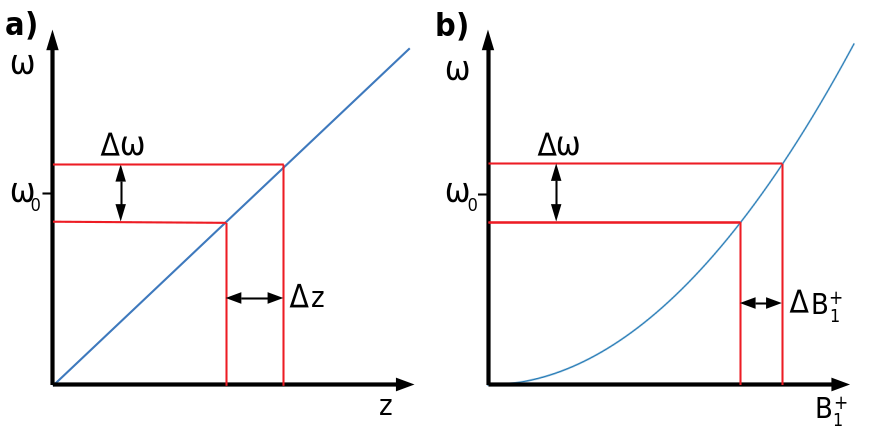
\includegraphics[width=0.75\textwidth]{figures/intro_figure.png}
\caption{a) Conventional slice selection, in which a linear gradient in the $B_0$ field introduces a spatial variation in resonant frequencies. 
When paired with a frequency-selective excitation pulse with center frequency $\omega_0$ and bandwidth $\Delta z$ a spatial slice of thickness $\Delta z$ is excited. 
b) Bloch-Siegert shift-localized slice selection, 
When paired with a frequency-selective excitation pulse, this results in the excitation of spins across a range $\Delta B_1^+$, which can be mapped to space using an amplitude gradient transmit coil.}
\label{fig:intro}
\end{figure}

%%%%%% FIGURE 2 %%%%%%%
\begin{figure}[h]
\centering
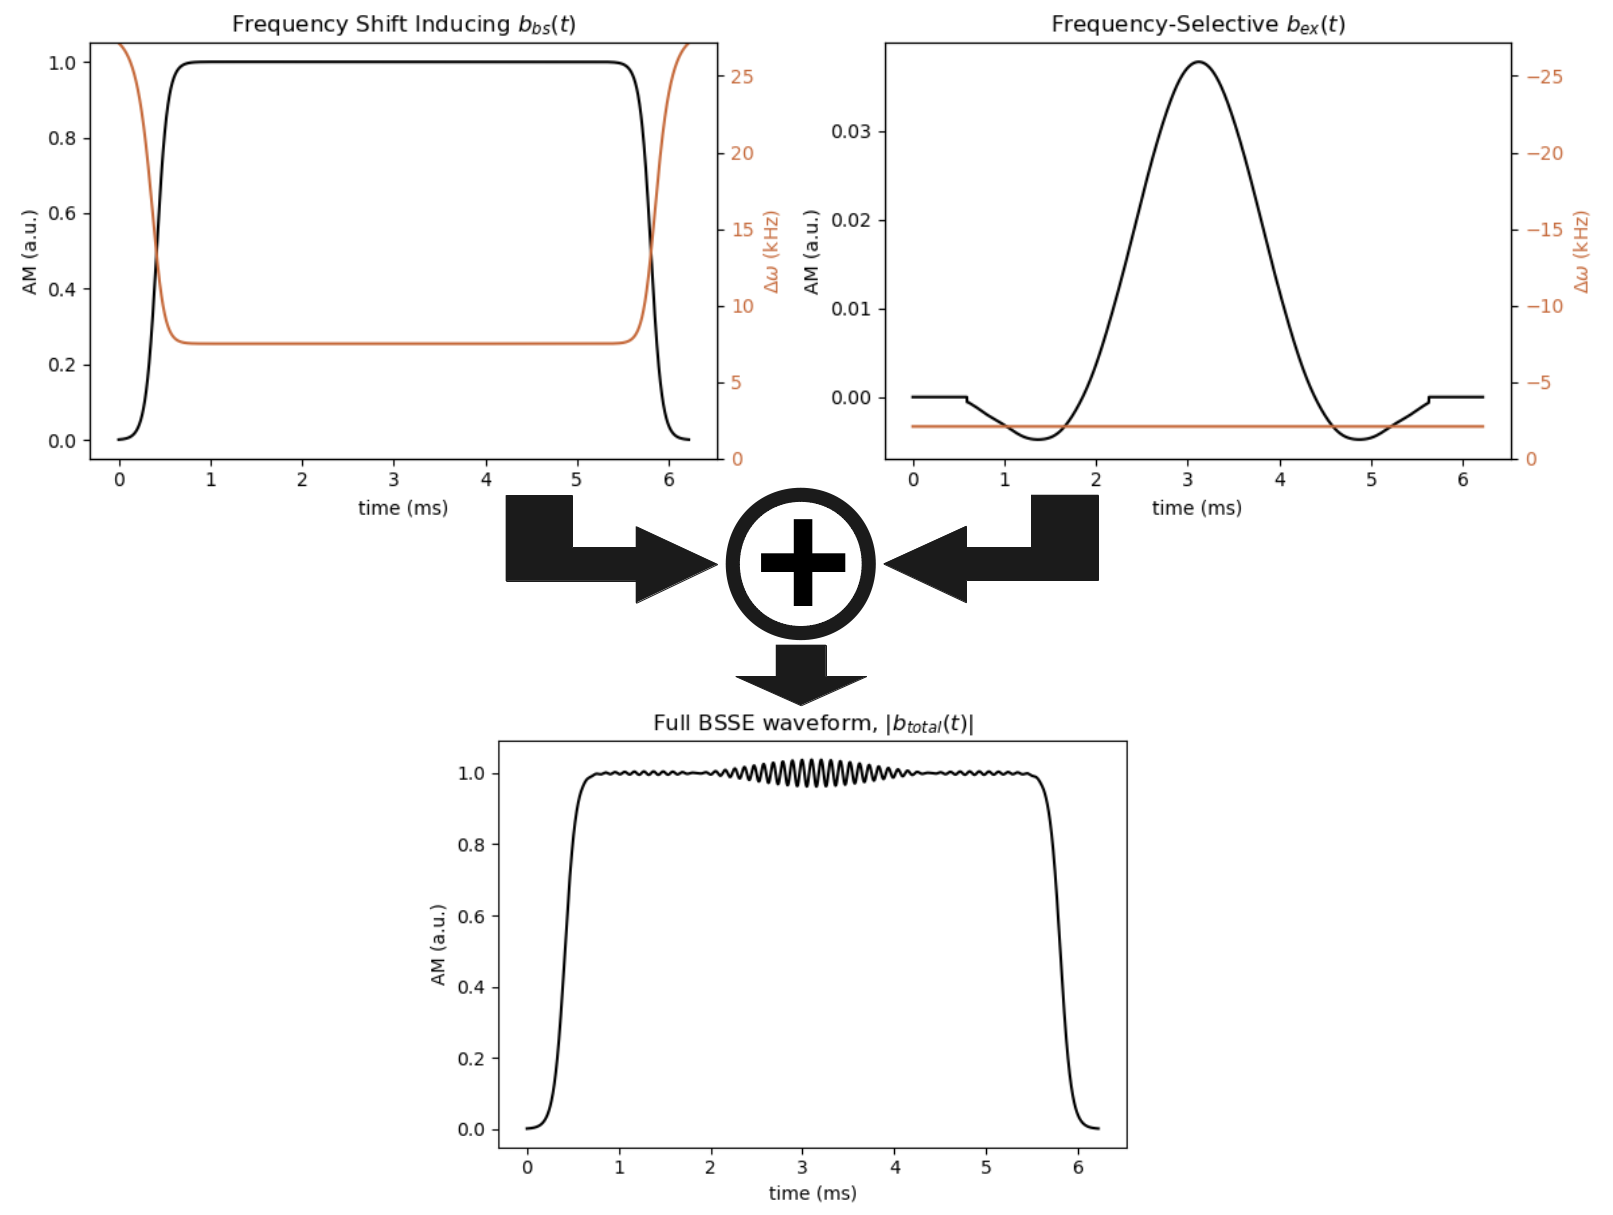
\includegraphics[width=1.1\textwidth]{figures/pulse_construction.png}
\caption{Construction of the full $b_{total}(t)$ BSSE RF pulse. The Bloch-siegert shift producing pulse $b_{bs}(t)$ (top left) and slice-selective pulse $b_{ex}(t)$ (top right) are designed independently and summed into the full BSSE waveform $b_{total}(t)$ (bottom). $b_{bs}(t)$ has Fermi AM (black) and adiabatic frequency sweeps towards and away from a constant frequency offset $\omega_{off}$ (orange). $b_{ex}(t)$ has SLR-designed AM (black) and a constant frequency offset (orange). 
Note that the amplitude of the BS waveform is generally much larger than that of the SS waveform; in $|b_{total}(t)|$, $b_{ex}(t)$ is visible as a small ripple present in the plateau of the Fermi waveform.}
\label{fig:alg}
\end{figure}

%%%%%% FIGURE 3 %%%%%%%
\begin{figure}[h]
\centering
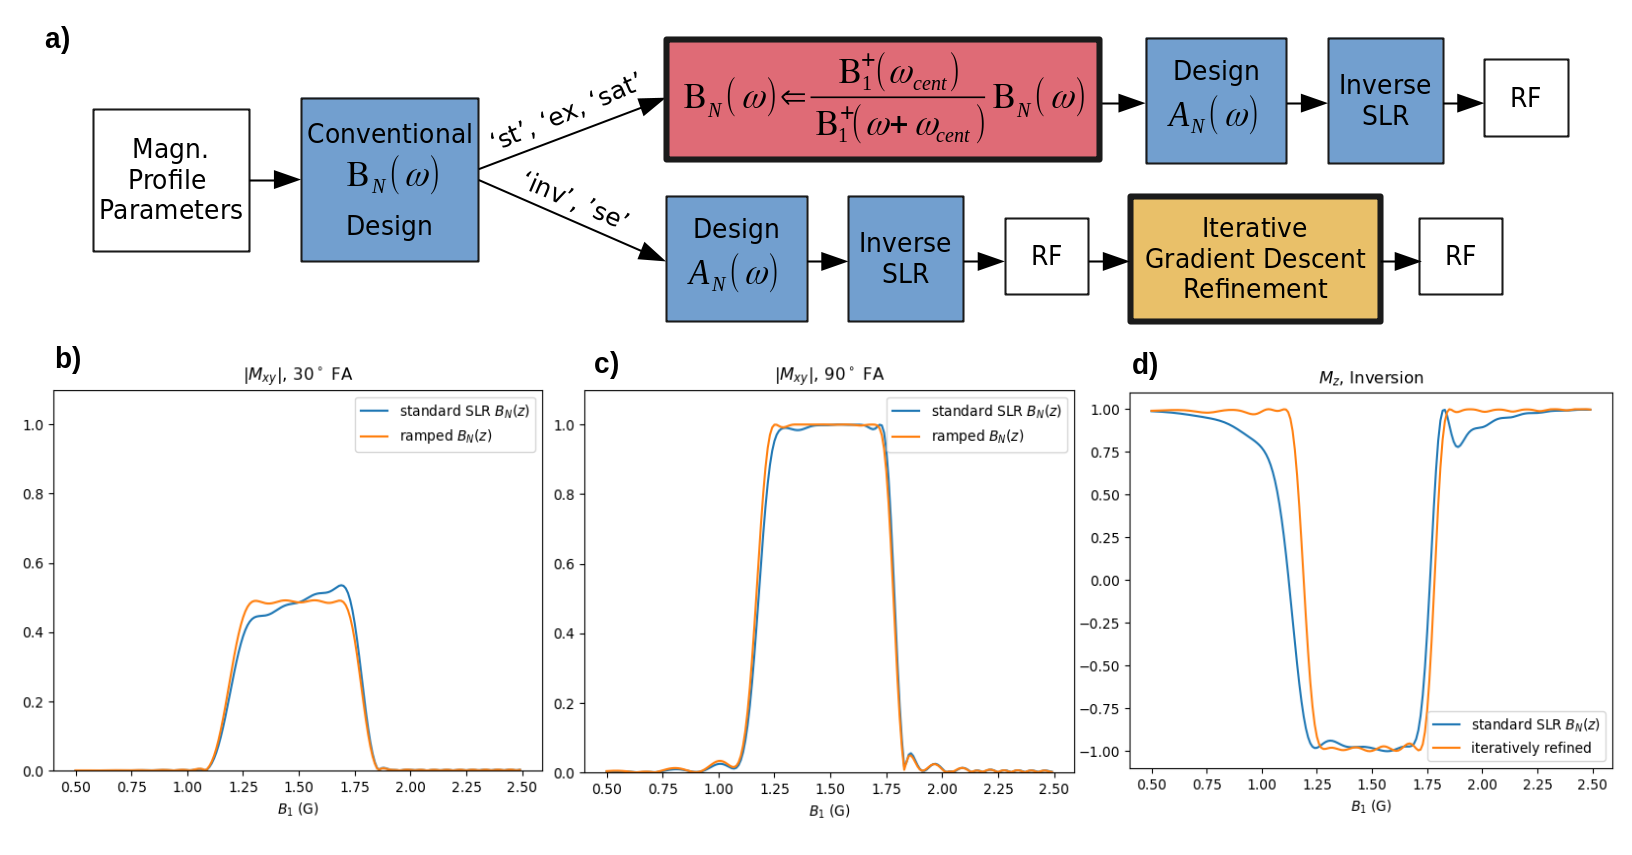
\includegraphics[width=1\textwidth]{figures/beta_filt_flowchart.png}
\caption{a) SLR design algorithm to compensate for a sloped excitation profile across $B_1^+$. In the case of small-tip (`st') or 90° (`ex', `sat') excitation, a
pointwise scaling of the $B_N (\omega)$ profile is sufficient. 
For an inversion (`inv') or refocusing (`se') pulse, iterative refinement is required. 
b) Uncorrected and corrected 30°, PBC = 1.4 G, PBW = 0.6 G, $T_{ex}B=8$ excitation.
c) Uncorrected and corrected 90° excitation. 
d) Uncorrected and corrected inversion profile after
autodifferentiated gradient descent optimization of the pulse with respect to its magnetization profile, Iterative refinement corrected the highly distorted transition bands of the profile.}
\label{fig:ramp}
\end{figure}

%%%%%% FIGURE 4 %%%%%%%
\begin{figure}[h]
\centering
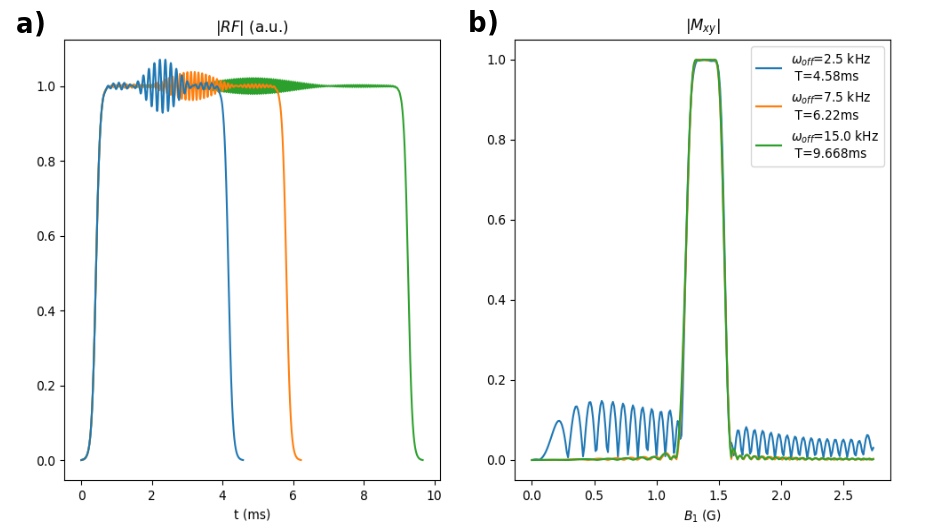
\includegraphics[width=1\textwidth]{figures/bs_offset_comparison_processed.png}
\caption{Comparison of magnetization profiles produces by BSSE pulses with varying $\omega_{off}$. 
a) Increasing $\omega_{off}$ increases minimum pulse duration, 
due to the reduced bandwidth produced by the smaller Bloch-Siegert shift across $B_1^+$. 
b) Larger offsets can help to reduce out-of band excitation. 
A pulse with $\omega_{off}$ = 2.5 kHz produces a substantial amount of out-of-band excitation, 
which is reduced to within design specifications when $\omega_{off} \rightarrow$ 7.5 kHz. 
Continuing to increase $\omega_{off}$ to 15.0 kHz did not further improve the profile.}
\label{fig:bsse_offres_comp}
\end{figure}


%%%%%% FIGURE 5 %%%%%%%
\begin{figure}[h]
\centering
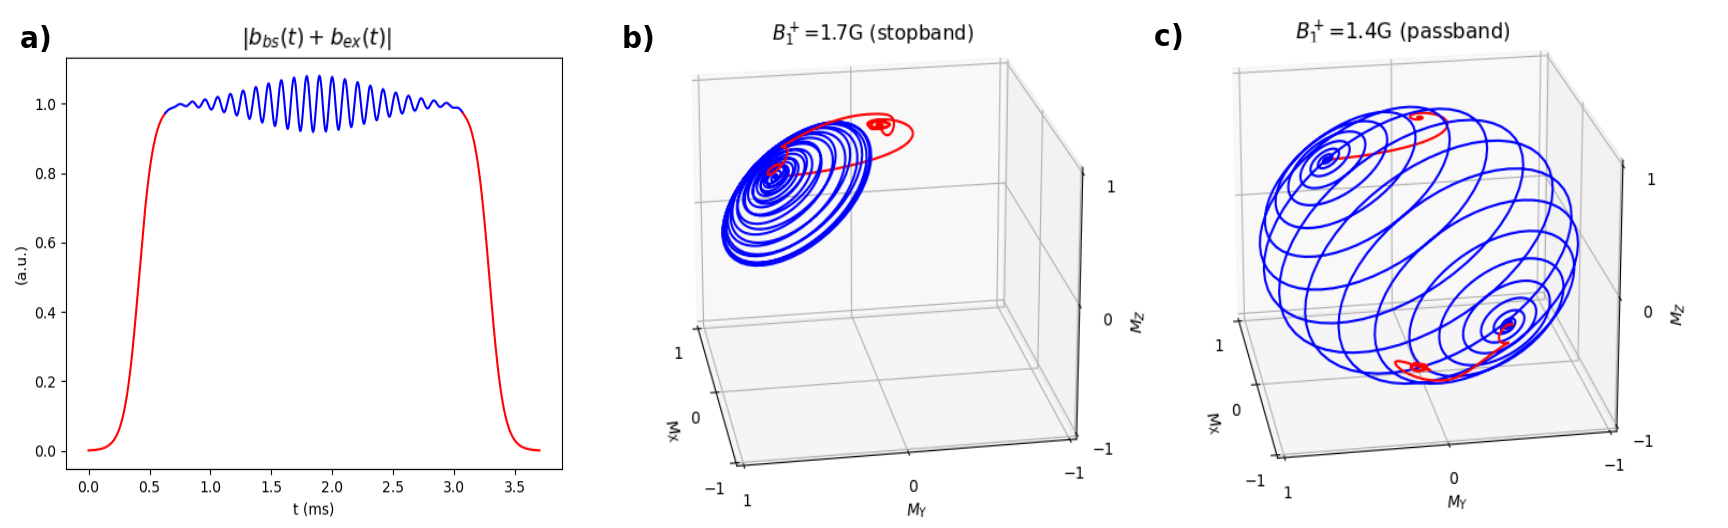
\includegraphics[width=1.1\textwidth]{figures/trajectory_figure.png}
\caption{a) Magnitude of a $T = 3.7$ ms BSSE inversion pulse. 
The pulse is colored red during the adiabatic frequency sweeps when $\bext = 0$, and blue during the constant portion of $\bbst$ when $\bext \neq 0$. 
b) Motion of the net magnetization vector in the $\omega_{off}$ rotating frame for a stopband isochromat. 
The simulation timestep was 4 $\mu$s. At the end of the pulse, magnetization is essentially unperturbed.
c) Motion of the net magnetization vector in the $\omega_{off}$ rotating frame for a passband isochromat. 
At the end of the pulse, magnetization is successfully inverted.}
\label{fig:motion}
\end{figure}

%%%%%% FIGURE 6 %%%%%%%
\begin{figure}[h]
\centering
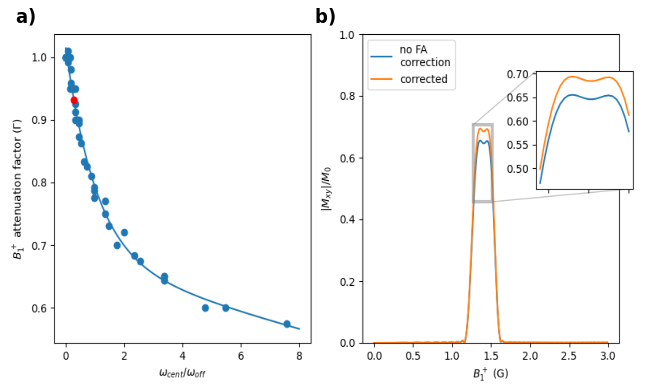
\includegraphics[width=1.\textwidth]{figures/correction_fact_processed_fa_only.png}
\caption{a) Flip angle attenuation factor versus $ \omega_{cent}/\omega_{off}$.
Data points are empirical correction factors found through simulation, 
with an exponential fit to the data shown as a continuous line. 
The red dot indicates the parameters of the pulse simulated in (b)
b) Excited slice profile of a PBC =1.4 Gauss, PBW = 0.3 Gauss, 
$45^\circ$, $\omega_{off}$=7.5 kHz pulse with and without the empirical FA correction. For this pulse, $\omega_{cent}/\omega_{off}$ = 0.279, which the model predicts will result in a flip angle attenuation of $6.9\%$ if uncorrected.
Applying the correction improves the effective flip angle of the pulse, bringing it closer to the anticipated $|M_{xy}|/M_0 = 0.7$
}
\label{fig:corrs}
\end{figure}

%%%%%% FIGURE 7 %%%%%%%
\begin{figure}[h]
\centering
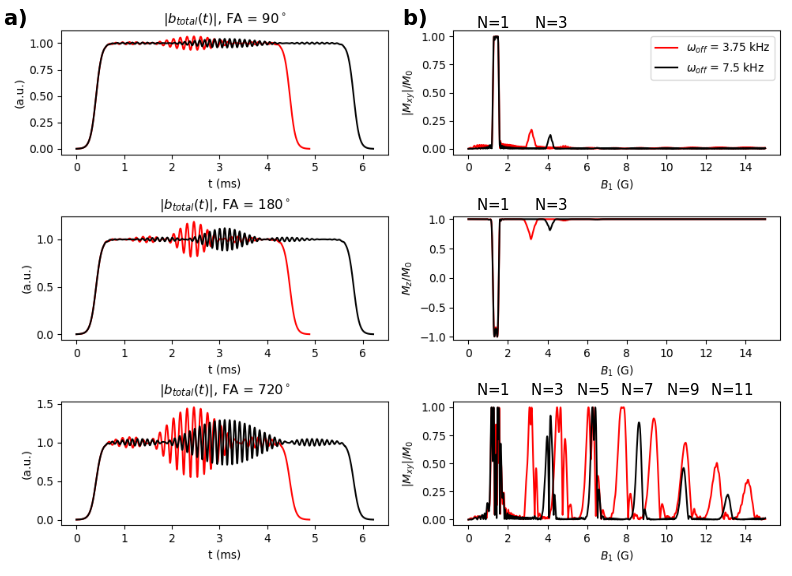
\includegraphics[width=1.1\textwidth]{figures/multiphoton_processed.png}
\caption{a) Magnitudes of $90^\circ$, $180^\circ$, and $720^\circ$ BSSE pulses with $\omega_{off}$ = 7.5 kHz (black) and $\omega_{off}$= 15.0 kHz (red). 
b) The corresponding simulated magnetization profiles. 
Multiphoton resonances are visible at the locations in $B_1^+$ predicted by Equation $\ref{eq:mp_b1}$. 
Increasing $\omega_{off}$ shifts resonances $N \geq 3$ upward in $B_1^+$.}
\label{fig:multiphoton}
\end{figure}

%% Comment: add legend


%%%%%% FIGURE 8 %%%%%%%
\begin{figure}[h]
\centering
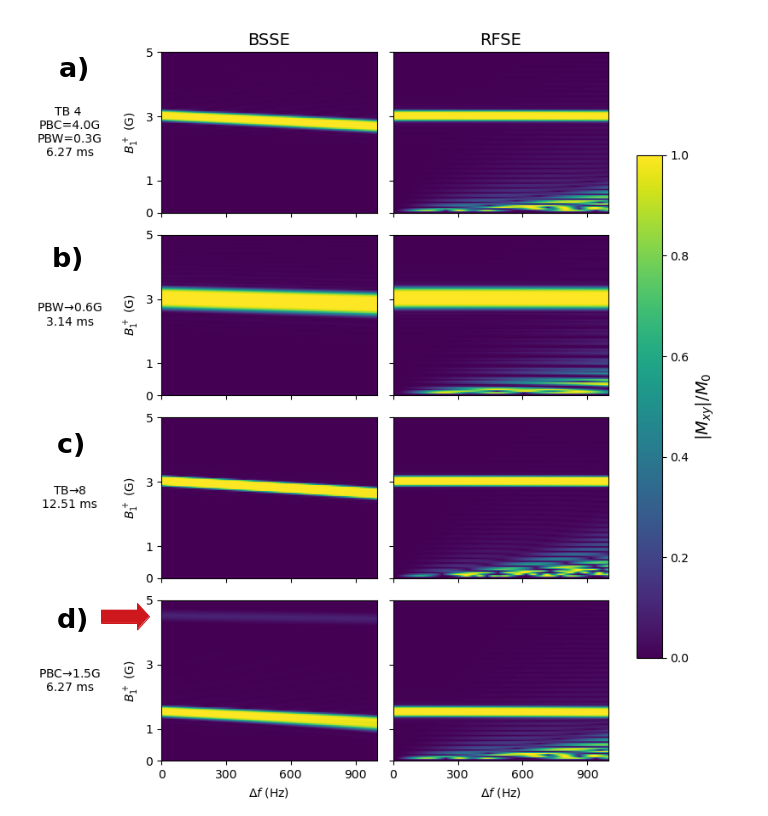
\includegraphics[width=0.8\textwidth]{figures/offres_processed.png}
\caption{Simulations of BSSE and RFSE pulse off-resonance sensitivity. 
a) Simulation of the ``base'' 6.27ms BSSE and RFSE pulses with TB=4, PBC=4.0G, PBW=0.3G, FA=90$^\circ$. 
$\omega_{off}$ was set to  16.37 kHz to match the RFSE pulse duration. 
b) Same as base pulse but with PBW set to 0.6 G. 
$\omega_{off}$ was set to 9.48 kHz to match durations. 
c) Same as base but with TB set to 8. 
$\omega_{off}$ was set to 19.25 kHz to match durations. 
d) Same as base but with PBC set to 1.5 G. 
$\omega_{off}$ was set to 8.17 kHz to match durations.
In all cases, the BSSE magnetization profiles show a bulk shift in the magnetization profile with increasing off-resonance. 
The red arrow in d) shows the location of an $N=3$ multiphoton resonance. 
This multiphoton resonance also experiences a bulk shift downward in $B_1^+$ with increasing off-resonance. 
The RFSE profiles show no bulk shift, but have substantial unintended excitation at low $B_1^+$.}
\label{fig:offres}
\end{figure}

%%%%%% FIGURE 9 %%%%%%%
\begin{figure}[h]
\centering
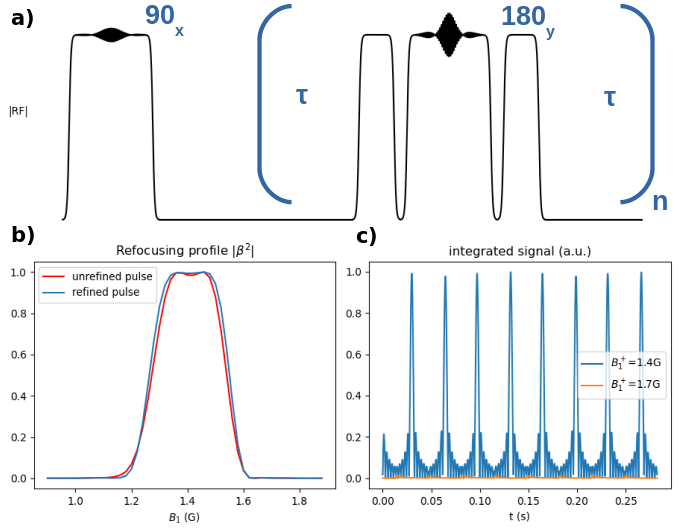
\includegraphics[width=1\textwidth]{figures/cpmg_oneb1_refined_processed.png}
\caption{BSSE Multi-echo CPMG pulse sequence. 
a) Pulse sequence diagram. A 90$^\circ$ excitation pulse was followed by a train of 180$^\circ$ pulses. 
The frequency-swept Fermi RF pulses of \S 2.1 were used in place of refocusing gradients. 
b) $|\beta^2|$ refocusing efficiency profile for the refocusing pulse. 
Refocusing was selective and nearly complete across the passband. 
The gradient descent-refined 180$^\circ$ pulse had a more selective and wider profile, 
although the unrefined pulse also performs well given the narrow PBW. 
c) Signal timecourse in the passband and stopband. 
Regularly spaced echos of uniform amplitude were produced in the passband.}
\label{fig:cpmg}
\end{figure}



%%%%%% FIGURE 10 %%%%%%%
\begin{figure}[h]
\centering
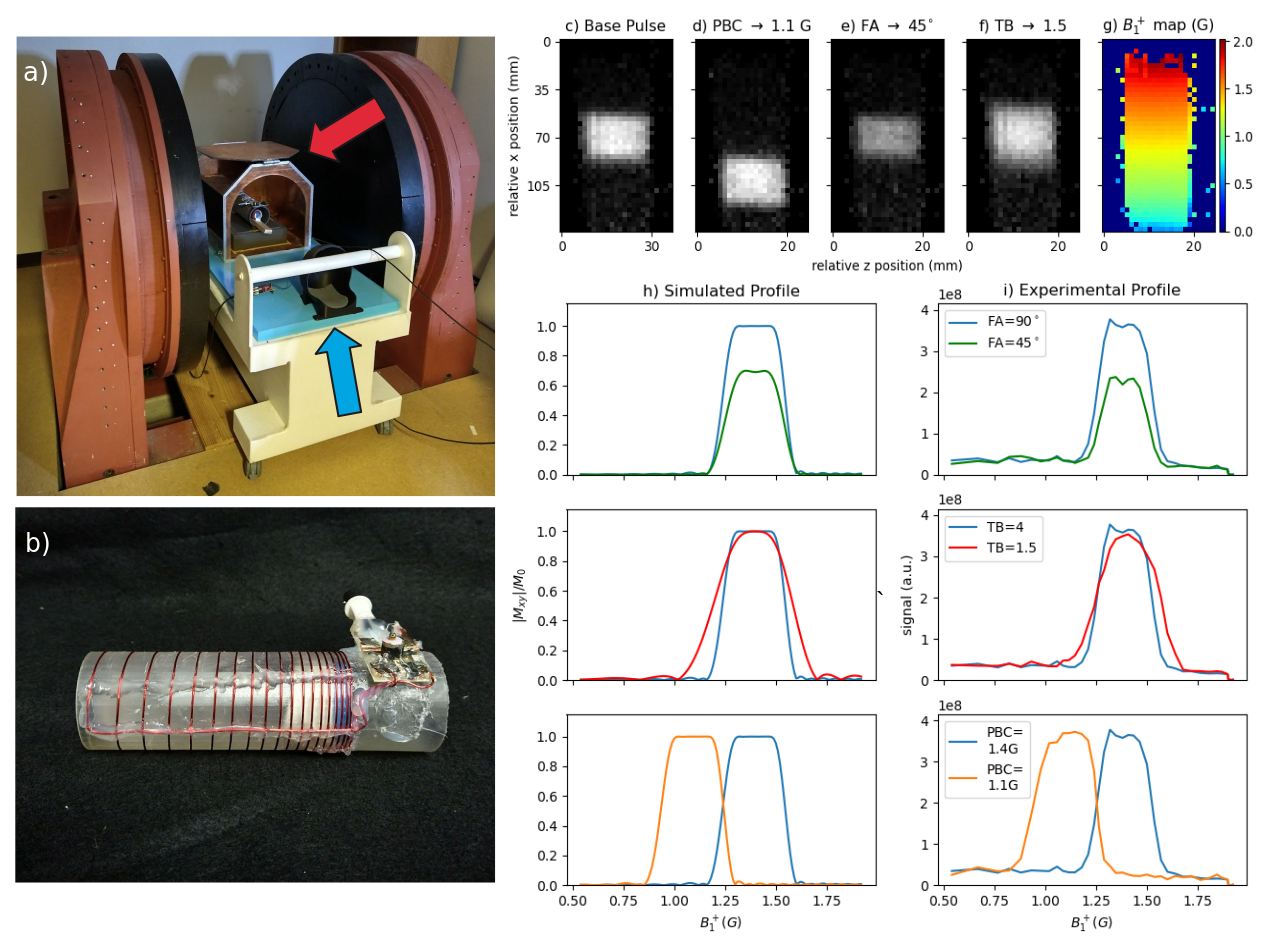
\includegraphics[width=1.1\textwidth]{figures/experimental_2D_processed_Rev2.png}
\caption{a) 47.5 mT permanent magnet system used for experimental results. A Faraday cage (red arrow) and pickup coil (blue arrow) are used to reduce EMI. b) variable-pitch T/R solenoid coil used in experiments. The tube phantom is placed inside in this image. c-f) middle slice of 3D GRE acquisition with varying BSSE excitation pulse. g) $B_1^^+$ map corresponding to the same slice h) 1D simulated profiles for the pulses, and i) corresponding experimental 1D profiles. The $45^\circ$ excitation (green) produces reduced signal intensity in relation to the $90^\circ$ excitation (blue). The $TB$=1.5 excitation (red) produces a profile with a broader transition region. Designing the pulse with PBC shifted to 1.1 G (orange) produces the corresponding change in the magnetization profile. 
}
\label{fig:exp}
\end{figure}

\renewcommand{\figurename}{Supporting Information Figure}
\renewcommand\thefigure{S\arabic{figure}}
\setcounter{figure}{0}

% %%%%%% FIGURE S1 %%%%%%%
% \begin{figure}[h]
% \centering
% 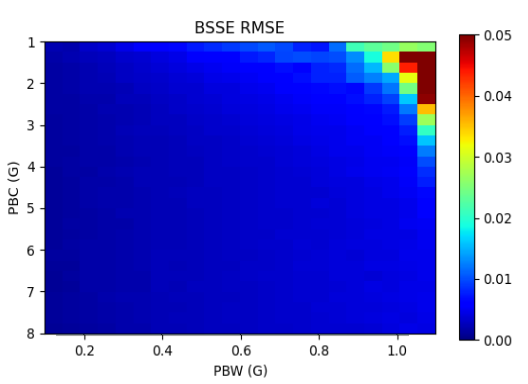
\includegraphics[width=0.8\textwidth]{figures/bsse_rmse.png}
% \caption{\textcolor{red}{WAG: Needs to be discussed in Results.} 
% BSSE magnetization profile RMSE for a pulse with $\omega_{off}$=7.5kHz, TB=4, FA=$90^\circ$. Across a broad range of PBW and PBC, the BSSE pulse has extremely low RMSE. However, in the regime in which the PBW becomes large relative to the PBC (top right), error sharply increases. This is primarily due to the nonlinearity of the Bloch-Siegert shift at low $B_1^+$}
% \label{fig:bsse_rmse}
% \end{figure}

%%%%%% FIGURE S1 %%%%%%%
\begin{figure}[h]
\centering
\includegraphics[width=1.1\textwidth]{figures/magmotion_appendix.gif}
\caption{ a) Magnitude of a $T = 3.7$ ms BSSE inversion pulse. 
The red trace is 10 $\mu$s long. 
b) Stopband magnetization trajectory in the $\omega_{off}$ rotating frame. 
The Simulation timestep was 4 $\mu$s.
c) Passband magnetization trajectory in the $\omega_{off}$ rotating frame.}
\label{fig:magmotion_animated}
\end{figure}



\end{document}
